              
% --------------------------------------------------------------
% This is all preamble stuff that you don't have to worry about.
% Head down to where it says "Start here"
% --------------------------------------------------------------
 
\documentclass[12pt]{article}
\usepackage{listings}
\usepackage{fancyvrb}
\usepackage{bera}

\usepackage[margin=1in]{geometry} 
\usepackage{amsmath,amsthm,amssymb}
\usepackage{url}
\usepackage{graphicx}
\usepackage{float}
\usepackage{paralist}
\setlength{\parindent}{0mm}
\newcommand{\N}{\mathbb{N}}
\newcommand{\Z}{\mathbb{Z}}
 
\newenvironment{theorem}[2][Theorem]{\begin{trivlist}
\item[\hskip \labelsep {\bfseries #1}\hskip \labelsep {\bfseries #2.}]}{\end{trivlist}}
\newenvironment{lemma}[2][Lemma]{\begin{trivlist}
\item[\hskip \labelsep {\bfseries #1}\hskip \labelsep {\bfseries #2.}]}{\end{trivlist}}
\newenvironment{exercise}[2][Exercise]{\begin{trivlist}
\item[\hskip \labelsep {\bfseries #1}\hskip \labelsep {\bfseries #2.}]}{\end{trivlist}}
\newenvironment{reflection}[2][Reflection]{\begin{trivlist}
\item[\hskip \labelsep {\bfseries #1}\hskip \labelsep {\bfseries #2.}]}{\end{trivlist}}
\newenvironment{proposition}[2][Proposition]{\begin{trivlist}
\item[\hskip \labelsep {\bfseries #1}\hskip \labelsep {\bfseries #2.}]}{\end{trivlist}}
\newenvironment{corollary}[2][Corollary]{\begin{trivlist}
\item[\hskip \labelsep {\bfseries #1}\hskip \labelsep {\bfseries #2.}]}{\end{trivlist}}
 
\begin{document}
 
% --------------------------------------------------------------
%                         Start here
% --------------------------------------------------------------
 
%\renewcommand{\qedsymbol}{\filledbox}
 
\title{\bf Fortran Modernisation Workshop \\ Exercises}

 
\maketitle

This exercise will involve modernising a legacy Fortran 77 code\footnote{\url{https://people.sc.fsu.edu/~jburkardt/f77_src/fd1d_heat_explicit/fd1d_heat_explicit.html}} to modern Fortran. The code solves the one dimensional heat diffusion equation:
\begin{equation} \label{fd1hd}
\frac{\partial H}{\partial t} - \kappa\frac{\partial^{2} H}{\partial x^{2}} = f(x)
\end{equation}
where $\kappa$ is the heat coefficient. Equation~(\ref{fd1hd}) describes the distribution of heat 
between $x_{\text{min}}$ and $x_{\text{max}}$ and uses the following explicit finite difference 
scheme to integrate in time:
\begin{align}
H^{(n+1)}_{i} & = H^{(n)}_{i} + \text{CFL}\big\{H^{(n)}_{i-1}-2H^{(n)}_{i} +
                      H^{(n)}_{i+1}\big\} + \Delta t f(x_{i}) \label{fd} \\
            \text{where CFL} & = \kappa\frac{\Delta t}{\Delta x^{2}} \label{cfl}
\end{align}
Equation~(\ref{cfl}) is known as the Courant-Friedrichs-Lewy coefficient which must satisfy
the condition $\text{CFL} > 0.5$ for~(\ref{fd}) to be stable. Don't worry if you do 
not know what all this means - the focus of the exercise is on Fortran programming. \\

The exercises are split into two parts: day one and day two. Set up Git:
\begin{Verbatim}[commandchars=\\\{\}]
git config --global user.name "\textit{firstname lastname}"
git config --global user.email \textit{firstname.lastname}@address.com
cd fmw_exercises
git init
git add .
git commit -m "initial version"
\end{Verbatim}
Replace the \textit{firstname} and \textit{lastname} with your name :-) The Git commands
will version control your code so you can see its revision history. Git will
be covered in the second day. Please put all your source code in the \texttt{src/}
directory. You can add a remote repository to your local repository using (replace \textit{username} and \textit{repo}
with your upstream username and repository name, respectively):
\begin{Verbatim}[commandchars=\\\{\}]
git remote add origin git@bitbucket.org:\textit{username}/\textit{repo}.git
git push origin master # after making changes to local repo
\end{Verbatim}
which you should do at the end of the workshop as the Linux machines will be cleaned 5 days after the workshop.
Day one exercises will include modernising an existing Fortran 77 code \texttt{fd1d\_heat\_explicit.f90} which
will be referred to the main program code. Day two exercises will involve the following topics:
\begin{enumerate}
\item Makefiles for Fortran codes;
\item Git source code version control system;
\item Fortran Documenter tool;
\item NetCDF file format for arrays;
\item In-memory visualisation using PLplot;
\item Unit testing with pFUnit;
\item Verification using CamFort.
\end{enumerate}
\newpage
\subsection*{Day One Exercises}
\setdefaultleftmargin{0pt}{}{}{}{}{}
\begin{enumerate}
\item Create a module \texttt{Types\_mod} and put it in the file \texttt{Types\_mod.f90} which 
contains the following numeric kind types:
\begin{verbatim}
use, intrinsic :: iso_fortran_env
integer, parameter :: SP = REAL32
integer, parameter :: DP = REAL64
integer, parameter :: SI = INT32
integer, parameter :: DI = INT64
\end{verbatim}
using the following module template: 
\begin{verbatim}
module Types_mod
   use, intrinsic :: iso_fortran_env

   implicit none
   ! everything is private unless otherwise stated
   private 
   public :: SP

   integer, parameter :: SP = REAL32
contains

end module Types_mod
\end{verbatim} \label{mod:temp}
\item Use the NAG compiler unifying precision feature to change \texttt{double precision} to \texttt{real(kind=DP)}
using the command (the output is a temporary file shown in italics which is then moved to the original file):
\begin{Verbatim}[commandchars=\\\{\}]
nagfor \textbf{=unifyprecision -pp_module=Types_mod -pp_name=DP} \textbackslash \\
  fd1d_heat_explicit.f90 -o \textit{fd1d_heat_explicit.f90_prs}
mv \textit{fd1d_heat_explicit.f90_prs} fd1d_heat_explicit.f90
\end{Verbatim}
\item In the main program code, use the NAG compiler polishing feature to:
\begin{enumerate}
\item change relational operators (e.g. \texttt{.LE.} to \texttt{<=})
\item capitalise keywords (e.g. \texttt{program} to \texttt{Program})
\item set the leftmost margin to zero
\item indentation to two spaces
\item add double colons for variable declarations (e.g. \texttt{integer i} to \texttt{integer ::\ i})
\item change old-style string declarations to modern Fortran string declarations (e.g. \texttt{character*11 ::\ str} to
\texttt{character(len=11) ::\ str}
\end{enumerate}
by using the command (the output is a temporary file shown in italics which is then moved to the original file):
\begin{Verbatim} [commandchars=\\\{\}]
nagfor \textbf{=polish -relational=F90+ -kwcase=C -margin=0 -indent=2} \textbackslash \\
  \textbf{-dcolon_in_decls=Insert -character_decl=Keywords} \textbackslash \\
  fd1d_heat_explicit.f90 -o \textit{fd1d_heat_explicit.f90_pol}
mv \textit{fd1d_heat_explicit.f90_pol} fd1d_heat_explicit.f90
\end{Verbatim}
\item In the main program code, change how parameters are declared, e.g.
\begin{Verbatim} [commandchars=\\\{\}]
integer t_num \\
parameter ( t_num = 201 ) \textit{! change to} \\
integer, parameter :: T_NUM = 201
\end{Verbatim}
And the same for the variable \texttt{X\_NUM}
\item In the main program code, change how constants are used, e.g. from \texttt{0.0D+00} to 
\texttt{0.0\_DP}
\item In the functions and subroutines, use the \texttt{intent} keyword for dummy arguments and properly
  scope the dummy arguments, e.g. \texttt{intent(in)} (read-only), \texttt{intent(out)} (write-only) or
  \texttt{intent(inout)} (read and write)
\item In the main program code, use dynamic memory allocation for the arrays \texttt{h(1:X\_NUM)}, 
\texttt{h\_new(1:X\_NUM)}, \texttt{hmat(1:X\_NUM,1:T\_NUM)}, \texttt{t(1:T\_NUM)}, \texttt{x(1:X\_NUM)}. Check
the status of the dynamic memory allocation\label{dyn:memory}
\item At the end of the main program code, deallocate the arrays declared in step~\ref{dyn:memory}
\item In the functions and subroutines, remove the size of the array and use assumed shaped
arrays as dummy arguments:
\begin{itemize}
\item For the function \texttt{func( j, x\_num, x )} remove the \texttt{x\_num} argument and
replace the argument declaration to \texttt{real(kind=DP), dimension(:)\ ::\ x}. Make sure
the calling of \texttt{func( )} reflect this change
\item For the function \texttt{fd1d\_heat\_explicit( )} remove the \texttt{x\_num} argument
and ensure all arrays are declared as assumed shaped arrays. Use the automatic arrays feature in Fortran
to declare the array \texttt{f(:)} as \texttt{real(kind=DP) ::\ f(size(x))}
\item For the function \texttt{r8mat\_write( )} declare the arguments \texttt{m} and \texttt{n} as local variables
  and assign them
to \texttt{size( table(:, :), 1 )} and \texttt{size( table(:, :), 2 )}, respectively. Declare the argument \texttt{table(:, :)}
as an assumed shaped array
\item For the function \texttt{r8vec\_linspace( )} remove the argument \texttt{n} and declare the argument \texttt{a(:)} as
an assumed shaped array
\item For the function \texttt{r8vec\_write( )} remove the argument \texttt{n} and declared the argument \texttt{x(:)} as
an assumed shaped array
\end{itemize}
Use the \texttt{size( )} intrinsic function to get array dimensions. 
\item Compile both the main program and the created Fortran module:
\begin{verbatim}
nagfor -c Types_mod.f90
nagfor -c -I. fd1d_heat_explicit.f90
nagfor fd1d_heat_explicit.o Types_mod.o -o fd1d_heat_explicit.exe
./fd1d_heat_explicit.exe
\end{verbatim}
\item To test whether your code runs correctly execute:
\begin{verbatim}
diff h_test01.txt h_test01.txt_bak
\end{verbatim}
If the command outputs difference, then the refactoring introduced a bug.
\item Type \texttt{git diff fd1d\_heat\_explicit.f90} to see the refactored code. Stage and commit
the changes by typing: 
\begin{verbatim}
git add fd1d_heat_explicit.f90
git add Types_mod.f90
git commit -m "refactored Fortran 77 into modern Fortran"
\end{verbatim}
The following exercises will modularise the code and use the module template in
  question~\ref{mod:temp} for creating additional modules.
\item Create a module \texttt{RHS\_mod} and put it in the file \texttt{RHS\_mod.f90} and {\bf move} the 
Fortran function \texttt{func()} into \texttt{RHS\_mod} and declare it public. In the main program code, 
insert the line \texttt{use RHS\_mod} 
\item Create a module \texttt{CFL\_mod} and put it in the file \texttt{CFL\_mod.f90} and {\bf move} the
  Fortran function \texttt{fd1d\_heat\_explicit\_cfl( )} into \texttt{CFL\_mod} and declare it
  public. In the main program
code, insert the line \texttt{use CFL\_mod}
\item Create a module \texttt{IO\_mod} and put it in the file \texttt{IO\_mod.f90} and {\bf move}
  the Fortran functions \texttt{r8mat\_write( )}, \texttt{r8vec\_linspace( )} and \texttt{r8vec\_write( )}
  into \texttt{IO\_mod} and declare them public. In the main program code, insert the line \texttt{use IO\_mod}
\item Create a module \texttt{Solver\_mod} and put it in the file \texttt{Solver\_mod.f90} and {\bf move} the
  Fortran function \texttt{fd1d\_heat\_explicit( )} into \texttt{Sover\_mod} and declare it public. In the main
  program code, insert the line \texttt{use Solver\_mod}
\item Compile the recently created modules:
\begin{verbatim}
nagfor -c RHS_mod.f90
nagfor -c CFL_mod.f90
nagfor -c IO_mod.f90
nagfor -c Solver_mod.f90
nagfor -c -I. fd1d_heat_explicit.f90
nagfor fd1d_heat_explicit.o Types_mod.o RHS_mod.o CFL_mod.o IO_mod.o \
         Solver_mod.o -o fd1d_heat_explicit.exe
./fd1d_heat_explicit.exe
\end{verbatim}
\item To test whether your code runs correctly execute:
\begin{verbatim}
diff h_test01.txt h_test01.txt_bak
\end{verbatim}
If the command outputs difference, then the refactoring introduced a bug.
\item Add the newly created module files into Git and stage the changed main program for a
another Git commit:
\begin{verbatim}
git add RHS_mod.f90 CFL_mod.f90 IO_mod.f90 Solver_mod.f90
git add fd1d_heat_explicit.f90
git commit -m "modularised RHS, CFL, IO and Solver"
\end{verbatim}
%
\end{enumerate}
\newpage
\subsection*{Day Two Exercises}
\begin{enumerate}
\item Write a Makefile for the Fortran code produced on day one in the same directory as the source
  code (\texttt{src/}) using the dependency graph in Figure~\ref{make_depend:eps}
\begin{figure}[H]
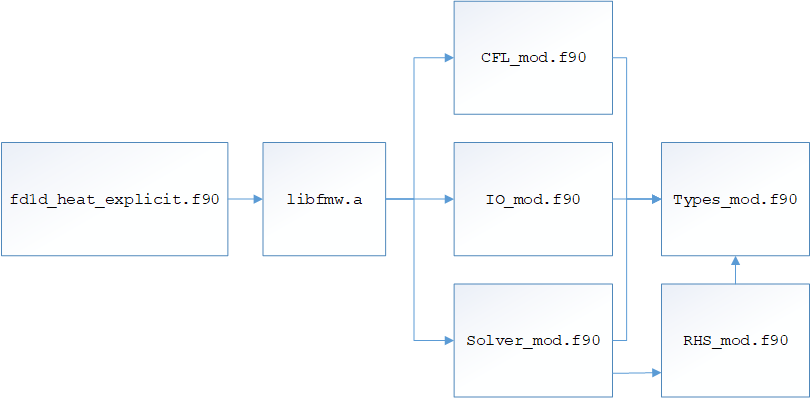
\includegraphics[height=6cm]{make_depend.png}
\caption{Dependency graph for Makefile}
\label{make_depend:eps}
\end{figure}
You can use the command:
\begin{verbatim}
makedepf90 *.f90
\end{verbatim}
to create the Makefile dependencies and then create the commands
\item Add a \texttt{clean} target which cleans the build:
\begin{verbatim}
.PHONY: clean

clean:
        rm -f *.mod *.o *.png *.exe *.a
\end{verbatim}
Remember to precede the commands with the tab
\item Create a static library containing all the module object files:
\begin{verbatim}
ar rcs libfmw.a CFL_mod.o IO_mod.o RHS_mod.o Solver_mod.o Types_mod.o
\end{verbatim}
In the Makefile, use the static library \texttt{libfmw.a} in the link stage to create the final executable. The link line for
linking \texttt{libfmw.a} is \texttt{-L. -lfmw}
\begin{enumerate}
\item After creating your Makefile, type \texttt{make -n} to see what commands will be executed without executing
your commands, which is useful for debugging
\item Then type \texttt{make} to build your code 
\item After creating the Makefile, add it to git using \texttt{git add Makefile}
\item Use the Linux command: 
\begin{verbatim}
nm libfmw.a
\end{verbatim}
which shows the symbols listed in the library just created. The symbol type field (second field) shows
\texttt{T} for the symbol being defined in the library and \texttt{U} being undefined but being called by the library. 
\end{enumerate}
\item This task will cover Git in a bit more detail.
\begin{enumerate}
\item Type \texttt{git status} which will list the status of all the files. Notice that the object 
files (\texttt{*.o}), Fortran module files (\texttt{*.mod}) and executable files (\texttt{*.exe}) are listed as 
untracked files. These files need not be version controlled as they can be recreated
\item Create the file \texttt{.gitignore} in the root directory (\texttt{fmw\_exercises/}). This configuration file will 
specify which files {\bf not to version control}, e.g. object files, executable files or any file that can
be recreated. Add the following extensions in the ignore file:
\begin{verbatim}
*.o
*.mod
*.exe
*.nc
*.dat
*.a
*.mp4
doc/
\end{verbatim}
\item The \texttt{.gitignore} file also needs to be version controlled using \texttt{git add .gitignore}
\item Browse the commit history of all the Fortran files created using \texttt{git log}
\end{enumerate}
\item Edit the template Fortran Documenter configuration file \texttt{fmw.md} in the root directory
(\texttt{fmw\_exercises/}) and set the following options:
\begin{center}
\begin{tabular}{| c | c |} \hline
{\bf Option} & {\bf Value} \\ \hline
\texttt{project:} & \texttt{1D heat equation} \\ \hline
\texttt{src\_dir:} & \texttt{./src} \\ \hline
\texttt{output\_dir:} & \texttt{./doc} \\ \hline
\texttt{summary:} & \texttt{Fortran Workshop} \\ \hline
\texttt{author:} & \texttt{Your name} \\ \hline
\texttt{docmark:} & \texttt{!} \\ \hline
\texttt{predocmark:} & \texttt{>} \\ \hline
\texttt{display:} & \texttt{public} \\ 
                  & \texttt{protected} \\ 
                  & \texttt{private} \\ \hline
\texttt{source:} & \texttt{true} \\ \hline
\texttt{graph:} & \texttt{true} \\ \hline
\texttt{search:} & \texttt{true} \\ \hline
\texttt{version:} & \texttt{1.1.1} \\ \hline
\end{tabular}
\end{center}
Note that the values for the \texttt{display} option must be on separate lines.
After the last option in the above table, leave an empty space and create \texttt{@Note} and \texttt{@Bug}
sections and add any text that describes your code.
\item On line 1 of the file \texttt{fd1d\_heat\_explicit.f90} add the following documentation:
\begin{Verbatim} [commandchars=\\\{\}]
!> \textit{<Your name>, <Your affiliation>}
!> Solves the one dimensional heat diffusion equation
!> \( \frac{\partial H}{\partial t} 
!>     - \kappa\frac{\partial^{2} H}{\partial x^{2}} = f(x) \)
\end{Verbatim}
\item On line 1 of the module file \texttt{CFL\_mod.f90} add the following comments:
\begin{verbatim}
!> this module calculates the CFL number
\end{verbatim}
In the same module file and for the subroutine \texttt{fd1d\_heat\_explicit\_cfl( )}, add
the following comments before the appropriate code lines:
\begin{verbatim}
!> calculates the CFL number  
!> \( \text{CFL} = \kappa\frac{\Delta t}{\Delta x^2} \)
subroutine fd1d_heat_explicit_cfl( )

!> calculated CFL number
real(KIND=DP), intent(inout) :: cfl
!> the heat constant \( \kappa \)
real(KIND=DP), intent(in) :: k
!> t_max upper bound of t-axis
real(KIND=DP), intent(in) :: t_max
!> lower bound of t-axis
real(KIND=DP), intent(in) :: t_min
!> number of intervals in t-axis
integer(KIND=SI), intent(in) :: t_num
!> upper bound of x-axis
real(KIND=DP), intent(in) :: x_max
!> x_min lower bound of x-axis
real(KIND=DP), intent(in) :: x_min
!> number of intervals in x-axis
integer(KIND=SI), intent(in) :: x_num
\end{verbatim}

Run the FORD command \texttt{ford fmw.md} and then load the file \texttt{doc/index.html} in any Web browser
to browse the source code documentation. Or, copy the directory \texttt{doc/} to your laptop to view the
code documentation.
\begin{enumerate}
\item Click on \texttt{Program} which displays the module dependency graph as well as the call graph. The
  local variables and the source code is also displayed;
\item The text also contains the LaTeX equation:
\begin{equation}
\frac{\partial H}{\partial t} - \kappa\frac{\partial^{2} H}{\partial x^{2}} = f(x)
\end{equation}
\item Have a browse around the other links to familiarise yourself with Fortran Documenter;
\item After the workshop has ended, do the same for the remaining module files 
(i.e. \texttt{IO\_mod.f90}, \texttt{RHS\_mod.f90}, \texttt{Solver\_mod.f90}, \texttt{Types\_mod.f90})
\item Commit the changed files in Git:
\begin{verbatim}
git add fd1d_heat_explicit.f90 CFL_mod.f90 fmw.md
git commit -m "added FORD documentation in source code"
\end{verbatim}
\end{enumerate}
\item The following exercises will involve using the NetCDF API by writing the
  \texttt{x(:)}, \texttt{t(:)} and \texttt{hmat(:, :)} varaibles in one file with meta-data. 
Please refer to the NetCDF documentation\footnote{~\url{http://www.nag.co.uk/market/training/fortran-workshop/netcdf-f90.pdf}} for the details of the API. Use the following process when creating NetCDF files for writing:
\begin{itemize}
\item\texttt{NF90\_CREATE( )} to create the file and enter define mode
\item\texttt{NF90\_DEF\_DIM( )} to create the $x$ and $t$ dimensions
\item\texttt{NF90\_DEF\_VAR( )} to create the \texttt{x(:)} (variable name \texttt{x-range}), \texttt{t(:)} (variable name
  \texttt{t-range}) and \texttt{table(:, :)} (variable name \texttt{solution}) variables
\item\texttt{NF90\_PUT\_ATT( )} to put global and dimension attributes
\item\texttt{NF90\_ENDDEF( )} to end define mode and to enter data mode
\item\texttt{NF90\_PUT\_VAR( )} to write the data to the file
\item\texttt{NF90\_CLOSE( )} to close the file
\end{itemize}
\begin{enumerate}
\item Open the file \texttt{IO\_mod.f90} and add the line \texttt{use netcdf}
\item Open the main program code \texttt{fd1d\_heat\_explicit.f90} and pass the arguments \texttt{x(:)} and
  \texttt{t(:)} into the subroutine call \texttt{r8mat\_write( )} and change the file name from \texttt{h\_test01.txt}
  to \texttt{h\_test01.nc} - the file extension \texttt{.nc} is used to denote NetCDF files
\item Comment out the two \texttt{r8vec\_write( )} subroutine calls
\item Edit the subroutine \texttt{r8mat\_write} and add the dummy arguments:
\begin{verbatim}
real(kind=DP), dimension(:), intent(in) :: x
real(kind=DP), dimension(:), intent(in) :: t
\end{verbatim}
\item When in define mode, add the following meta data using \texttt{NF90\_GLOBAL} for \texttt{varid} argument:
  \begin{enumerate}
  \item\texttt{"purpose" = "Fortran workshop"}
  \item\texttt{"name" = "<Your name>"}
  \item\texttt{"institution" = "<Your university>"} 
  \end{enumerate}
\item In the subroutine \texttt{r8mat\_write( )} write the one-dimensional arrays \texttt{x(:)} and \texttt{t(:)} and the
  two-dimensional array \texttt{table(:, :)} into a NetCDF file
\item To compile the remember to add the flag in your Makefile:
\begin{verbatim}
-I/usr/local/netcdf-4.6.1/include
\end{verbatim}
\item To do the final link, remember to add the link flag: 
\begin{verbatim}
-L/usr/local/netcdf-4.6.1/lib -lnetcdff -lnetcdf
\end{verbatim}
Note that the ordering of the flags is crucial (\texttt{netcdff} calls \texttt{netcdf} so this ordering is required).
The library \texttt{netcdff} contains the Fortran bindings and \texttt{netcdf} is the actual implementation in the
C language
\item After executing your code, you can view the contents of the NetCDF file using \texttt{ncdump h\_test01.nc | less}
\item To verify whether your code works correctly, compare the created NetCDF file with the correct NetCDF file:
\begin{verbatim}
ncdiff --overwrite h_test01.nc h_test01.nc.valid -o diff.nc
ncwa -y max --overwrite diff.nc out.nc
ncdump out.nc | grep "solution ="
\end{verbatim}
The last command should show \texttt{0} for the \texttt{solution} NetCDF variable
\end{enumerate}
\item The following exercises will allow you to visualise the solution at every 10 time steps using the PLplot
visualisation library. Please refer to Section 2 of the PLplot
documentation\footnote{\url{http://www.nag.co.uk/market/training/fortran-workshop/plplot-5.11.1.pdf}} for
further information. \\

The visualistion will be done in the main program \texttt{fd1d\_heat\_explicit.f90} using the
following sequence of subroutine calls from within the main time loop:
\begin{itemize}
\item\texttt{PLSFNAM( )} to set the output file name 
\item\texttt{PLSDEV( )} to set the output device to use. Set this to \texttt{"pngcairo"} which
will save the images in the portable network graphics format
\item\texttt{PLINIT( )} to initialise PLplot
\item\texttt{PLENV( )} to set the $x$- and $y$-range
\item\texttt{PLLAB( )} to set the $x$ and $y$ labels, and the title of the graph
\item\texttt{PLLINE( )} to set the $x$ and $y$ values which will be represented by the
  arrays \texttt{x(:)} and \texttt{h\_new(:)}, respectively
\item\texttt{PLEND( )} to finalise PLplot
\end{itemize}  
\begin{enumerate}
\item In the main program code, add the line \texttt{use plplot} so that PLplot features can be
used
\item In the main time loop create an IF branch which is executed at every 10 time steps
using the Fortran intrinsic function \texttt{mod( )}
\item Create a string for the filename which includes the time step, e.g. 
\texttt{image001.png}
\item From the above list of PLplot subroutine calls, create the PNG file of the
current time step
\item To compile the code, add the flag:
\begin{verbatim}
-I/usr/local/plplot-5.13.0/lib/fortran/modules/plplot
\end{verbatim}
The include path contains the Fortran module files for PLplot;
\item To link the code to the PLplot libraries, use the link flags
\begin{verbatim}
-L/usr/local/plplot-5.13.0/lib -lplplotfortran -lplplot
\end{verbatim}
Note that the ordering of the link flags is crucial (\texttt{plplotfortran} calls \texttt{plplot}). The
library \texttt{plplotfortran} contains the Fortran bindings and \texttt{plplot} is the actual
implementation in the C language
\item Then execute your code to create the PNG image of the solution at different time steps
  (\texttt{./fd1d\_heat\_explicit.exe}) which should create PNG files for time steps $n = 10,20,\ldots, 200$, e.g.
  \texttt{fd1d\_heat\_explicit\_00010.png}
\item Create a movie file with the list of images created using:
\begin{verbatim}
ffmpeg -f image2 -i fd1d_heat_explicit_%*.png fd1d_heat_explicit.mp4
\end{verbatim}
and view it using any video player
\end{enumerate}
\item Ensure the Makefile is updated to include the compile and link flags for NetCDF and PLplot
\item This exercise will involve creating pFUnit test pseudocodes. This exercise will only
test the CFL subroutine. 
\begin{enumerate}
\item Create the following test driver code which is in pseudo Fortran and name the file \texttt{testCFL.pf} 
which will test the \texttt{fd1d\_heat\_explicit\_cfl( )} subroutine:
\begin{verbatim}
@test
subroutine testCFL( )
  use pFUnit_mod
  use CFL_mod
  use Types_mod

  integer, parameter :: t_num = 201
  integer, parameter :: x_num = 21
  real(KIND=DP) :: k, x_min, x_max, t_min, t_max 
  real(KIND=DP) :: cfl, cfl_exact, tol

  tol = 0.0000001_DP
  cfl_exact = 0.32_DP
  k = 0.002_DP

  x_min = 0.0_DP
  x_max = 1.0_DP

  t_min = 0.0_DP
  t_max = 80.0_DP
  
  call fd1d_heat_explicit_cfl( k, t_num, t_min, t_max, &
                               x_num, x_min, x_max, cfl )

  @assertEqual( cfl, cfl_exact, tol )
end subroutine testCFL
\end{verbatim}
Place it in the same directory as the Fortran source code.
\item Create the test configuration file \texttt{testSuites.inc} which will tell pFUnit which tests to execute:
\begin{verbatim}
ADD_TEST_SUITE(testCFL_suite)
\end{verbatim}
\item To preprocess the pseudo Fortran test driver code to produce Fortran code (namely, \texttt{testCFL.F90}), type:
\begin{verbatim}
${PFUNIT}/bin/pFUnitParser.py testCFL.pf testCFL.F90 -I.
\end{verbatim}
where \texttt{\$PFUNIT} is the environment variable which points to the installation directory of pFUnit.
Note that the Fortran code must have the \texttt{.F90} extension as it still needs to be preprocessed
\item Then compile the created Fortran test driver code:
\begin{verbatim}
nagfor -I${PFUNIT}/mod -c testCFL.F90
\end{verbatim}
\item Then create the final test driver executable (\texttt{test.exe}):
\begin{verbatim}
nagfor -I$PFUNIT/mod $PFUNIT/include/driver.F90 \
       CFL_mod.o testCFL.o  -L$PFUNIT/lib -lpfunit -I. -o tests.exe 
\end{verbatim}
Note that \texttt{CFL\_mod.f90} must be compiled before the above command is executed
\item This command will create the \texttt{tests.exe} binary executable which needs to be executed
  and will print the result of the test, which is either a pass or fail, and the time it took to complete
  the test
\item Change the value \texttt{cfl\_exact} to \texttt{0.34\_DP} in the pseudo Fortran code and repeat
  steps (b), (c) and (d). Execute the \texttt{tests.exe} which should fail the test
\item Add the pFUnit commands listed above in the Makefile and call the target \texttt{pfunit}
\end{enumerate}
\item This exercise will involve using CamFort.
\begin{enumerate}
\item Use the CamFort command to obtain the stencil specification:
\begin{verbatim}
camfort stencils-infer Solver_mod.f90
\end{verbatim}
\item From the stencil specification obtained in the previous step, annotate the code:
\begin{verbatim}
h_new(j) = h(j) + dt * f(j) + cfl * (h(j-1) - 2.0_DP * h(j) + h(j+1))
\end{verbatim}
Remember to prefix every specification with \texttt{!= <specification>} 
\item Then use the CamFort command to verify the stencil specification:
\begin{verbatim}
camfort stencils-check Solver_mod.f90
\end{verbatim}
which should print \texttt{Correct} for every specification. 
\end{enumerate}
\end{enumerate}
\end{document}
